\documentclass[UTF8,a4paper,12pt]{ctexart}
\usepackage{amsmath,amssymb}
\usepackage{booktabs}
\usepackage{array}
\usepackage{geometry}
\usepackage{graphicx}
\usepackage{float}
\usepackage{hyperref}
\usepackage{longtable}
\usepackage{siunitx}
\geometry{left=2.5cm,right=2.5cm,top=2.5cm,bottom=2.5cm}
\graphicspath{{../figures/}{figures/}}
\hypersetup{colorlinks=true,linkcolor=black,citecolor=black,urlcolor=blue}
\ctexset{section={format=\Large\bfseries},subsection={format=\large\bfseries}}

\title{基于 UCI Adult 数据集的个人收入水平二分类预测}
\author{{高安程}\quad {2024302181042}}
\date{2026.5}

\begin{document}
\maketitle

\begin{abstract}
本次大作业以监督学习中的二分类问题为切入点，基于 UCI Adult/Census Income 数据集构建个人收入水平预测模型，目标是根据年龄、教育、职业、婚姻、工作时长等人口统计学与工作相关特征判断年收入是否超过 50,000 美元。清洗后数据集保留 45,222 条有效样本，并按 60\%/20\%/20\% 划分为训练集、验证集和测试集；StandardScaler 与 OneHotEncoder 均在训练集上拟合；同时，验证集和测试集沿用训练阶段得到的变换规则，以此控制数据泄漏风险。最终，MLP 在测试集上取得 0.8507 的 Accuracy 和 0.7947 的 Macro-F1，整体表现高于多数类预测、随机先验预测和逻辑回归三个参考模型。此外，我还通过控制变量法考察学习率与 Dropout 对收敛过程的影响，并结合混淆矩阵来分析高收入少数类样本更容易被误判的原因。
\end{abstract}

\textbf{关键词：}监督学习；二分类；UCI Adult；多层感知机；超参数分析；Macro-F1

\section{引言}
监督学习是我们这学期人工智能课中最基础也最常用的机器学习范式之一。其核心思想是在带标签样本上学习输入特征与目标变量之间的映射关系，并将这种映射推广到未见样本。分类任务是监督学习中最典型的任务类型，例如垃圾邮件识别、疾病风险预测、信用违约检测、图像类别识别等都可以被表述为分类问题。结合我本学期的实际学习情况，我将在报告中重点分析数据收集、预处理、构造对比模型、并对结果和算法进行解释的完整过程。

我选取经典的“个人收入水平预测”作为实操选题。该问题使用 UCI Machine Learning Repository 中的 Adult 数据集\cite{uciadult}，预测目标为年收入是否超过 50,000 美元。选择该数据集的原由简单如下：标签设定清楚，便于将任务定义为标准二分类问题；特征同时包含数值型变量和类别型变量，能够覆盖标准化、独热编码、缺失值处理等常见特征工程环节；样本标签呈现低收入类别占多数、高收入类别占少数的分布，但是，单独观察 Accuracy 容易遗漏少数类识别质量，因此需要结合 Macro-F1、Precision、Recall 和混淆矩阵进行评价。

先从 UCI 官方目录下载原始文件开始，随后合并原始训练文件与测试文件，并重新划分为训练集、验证集和测试集。在此基础上，先完成缺失值统计、标签分布和特征分布分析，再进入模型训练阶段。模型部分设置了多数类预测、随机先验预测和逻辑回归三个 baseline，并以多层感知机（MLP）作为主模型。随后的超参数分析围绕学习率和 Dropout 展开，通过训练曲线、混淆矩阵和指标表格共同判断模型的收敛状态与错误来源。

\section{监督学习技术综述}
监督学习的共同前提是训练集中每个样本都带有标签。给定输入特征 $x$ 和标签 $y$，算法希望学习函数 $f(x)$，使其在训练数据和未来数据上都能尽可能准确地预测标签。根据标签类型不同，监督学习通常分为分类和回归。分类任务的输出是离散类别，回归任务的输出是连续数值。本次报告主要关注二分类，即模型最终需要判断样本属于两个类别中的哪一个。

本学期涉及的常见的监督学习方法包括逻辑回归、决策树、随机森林、支持向量机、朴素贝叶斯、K 近邻和神经网络等。不同方法的建模假设、可解释性、计算成本和适用数据类型存在差异。表\ref{tab:methods}给出横向对比。
\begin{table}[H]
\centering
\caption{常见监督学习方法横向对比}
\label{tab:methods}
\begin{tabular}{p{2cm}p{3.2cm}p{3.4cm}p{3.9cm}}
\toprule
方法 & 基本假设或机制 & 优点 & 局限与适用场景 \\
\midrule
逻辑回归 & 线性决策边界，使用 Sigmoid 或 Softmax 输出概率 & 简单、稳定、可解释，适合强 baseline & 非线性表达能力受限，依赖特征工程 \\
决策树 & 通过特征阈值递归划分样本空间 & 可解释性强，能处理非线性关系 & 容易过拟合，单棵树稳定性有限 \\
随机森林 & 多棵决策树集成投票 & 泛化较好，对表格数据常有强表现 & 模型较大，解释单个预测较困难 \\
支持向量机 & 最大化分类间隔，可通过核函数非线性映射 & 小中规模数据上效果稳定 & 大样本训练成本较高，参数选择敏感 \\
朴素贝叶斯 & 条件独立假设下进行概率推断 & 训练快，适合文本等高维稀疏数据 & 独立性假设较强，复杂特征关系表达受限 \\
K 近邻 & 根据邻近样本标签投票 & 思想直观，无显式训练过程 & 预测成本高，对尺度和噪声敏感 \\
神经网络/MLP & 多层线性变换与非线性激活组合 & 表达能力强，可学习复杂非线性关系 & 需要调参，解释性较弱，表格数据收益依赖样本规模和特征表达 \\
\bottomrule
\end{tabular}
\end{table}

在本实验中，我选用逻辑回归作为传统线性强 baseline，由于 Adult 数据集中许多特征与收入之间存在近似单调或线性可分的关系，例如教育年限、资本收益和工作时长。从而，MLP 被选为主模型，其隐藏层能够组合多个特征，能学习线性模型表达能力受限的交互模式。由此也不难理解，“教育水平较高且每周工作时长较长且职业类型为专业技术”的组合，比任何单个特征更能指示高收入类别。

\section{MLP 技术深入分析}
多层感知机是一种前馈神经网络。给定输入向量 $x$，一层全连接网络可写为
\[
h = \sigma(Wx + b),
\]
其中 $W$ 是权重矩阵，$b$ 是偏置，$\sigma$ 是非线性激活函数。在仅堆叠线性变换的情况下，多层线性函数的复合仍可化简为一个线性函数；ReLU 等非线性激活使网络能够形成分段线性决策边界，因此成为 MLP 获得非线性表达能力的关键。网络采用两层隐藏层结构：

\[
\text{Input} \rightarrow \text{Linear(104,128)} \rightarrow \text{ReLU} \rightarrow \text{Dropout}\rightarrow \text{Linear(128,64)} \rightarrow \text{ReLU} 
\\
\rightarrow \text{Dropout}
\rightarrow \text{Linear(64,2)}.
\]

其中输入维度 104 来自 6 个数值特征和 8 个类别特征独热编码后的拼接结果。

本次实验采用两个 logits 并配合交叉熵损失来处理二分类任务。模型输出 $z_0,z_1$ 后，Softmax 将其转换为类别概率：
\[
p_i=\frac{e^{z_i}}{\sum_j e^{z_j}}.
\]
交叉熵损失为
\[
L=-\sum_i y_i\log p_i.
\]
当真实类别概率被模型赋得越低时，损失越大，反向传播会据此调整权重。反向传播的本质是链式法则：先计算输出层误差，再逐层向前传播梯度，最后使用优化器更新参数。实验使用 AdamW 优化器，它在 Adam 的自适应学习率基础上引入解耦权重衰减，有助于限制参数过大。

MLP 的优势体现在表达能力上。隐藏层可以自动组合特征并学习复杂非线性关系，参数数量、解释性、超参数选择和数据预处理也会同步影响实验结果。对于 Adult 这样的表格数据，模型收益取决于原始特征能否提供足够的交互信息、样本量能否支撑参数学习、类别特征独热编码能否保留有效结构，以及优化过程是否出现过拟合或欠拟合。

Dropout 是本实验使用的重要正则化方法\cite{srivastava2014dropout}。训练时，Dropout 以一定概率随机屏蔽隐藏层神经元，降低模型对少数特征组合的依赖程度。从优化角度看，它会改变每个 batch 中实际参与计算的隐藏单元集合，使参数更新受到更多扰动，从而提升模型对输入变化的适应能力。Dropout 取值过小会削弱正则化效果，取值过大会降低网络有效容量并引发欠拟合倾向。 

\section{应用设计与数据处理}
\subsection{数据来源与字段描述}
Adult 数据集由 Becker 和 Kohavi 整理，常用于收入预测研究\cite{kohavi1996scaling}。可以从 UCI 官方目录手动下载 \texttt{adult.data}、\texttt{adult.test} 和 \texttt{adult.names}，然后读取本地原始文件。原始数据共 48,842 条样本，清洗缺失值后保留 45,222 条。表\ref{tab:fields}列出字段。

\begin{table}[H]
\centering
\caption{Adult 数据集字段描述}
\label{tab:fields}
\begin{tabular}{p{3.2cm}p{2.2cm}p{7cm}}
\toprule
字段 & 类型 & 含义 \\
\midrule
age & 数值 & 年龄 \\
workclass & 类别 & 工作类型，如 Private、Self-emp 等 \\
fnlwgt & 数值 & 人口统计抽样权重 \\
education & 类别 & 教育阶段文本描述 \\
education-num & 数值 & 教育年限编码 \\
marital-status & 类别 & 婚姻状态 \\
occupation & 类别 & 职业类别 \\
relationship & 类别 & 家庭关系 \\
race & 类别 & 种族类别 \\
sex & 类别 & 性别 \\
capital-gain & 数值 & 资本收益 \\
capital-loss & 数值 & 资本损失 \\
hours-per-week & 数值 & 每周工作小时数 \\
native-country & 类别 & 出生国家或地区 \\
income & 标签 & 是否年收入超过 50K \\
\bottomrule
\end{tabular}
\end{table}

\subsection{清洗与探索性分析}
下载下来的原始文件中缺失值使用问号表示。代码读取时将 \texttt{?} 识别为缺失值，并统一清理字符串首尾空格。由于 \texttt{adult.test} 中标签末尾带句点，例如 \texttt{>50K.}，读取后需统一删除标签末尾句点，使训练和测试原始文件的标签格式保持一致。在缺失值处理上，考虑到剔除含问号的记录后仍有 45,222 条有效样本，样本规模足以支撑后续神经网络训练，最终采用直接删除缺失样本的保守策略。这种处理方式减少了插补算法带来的额外假设，也使清洗过程相对而言更容易复现。缺失值统计如表\ref{tab:missing}。

\begin{table}[H]
\centering
\caption{主要缺失值统计}
\label{tab:missing}
\begin{tabular}{lrr}
\toprule
字段 & 缺失数量 & 缺失比例 \\
\midrule
workclass & 2,799 & 5.73\% \\
occupation & 2,809 & 5.75\% \\
native-country & 857 & 1.75\% \\
其他字段 & 0 & 0.00\% \\
\bottomrule
\end{tabular}
\end{table}

图\ref{fig:label}显示标签分布。低收入类别占约 75.2\%，高收入类别占约 24.8\%，对应着明显的类别不均衡。模型若将全部样本预测为多数类，Accuracy 仍可达到约 0.752，此时高收入类别召回率为 0，Macro-F1 会显著下降。因此，我们需要同时关注 Accuracy 和 Macro-F1。图\ref{fig:numeric}展示年龄、教育年限和每周工作时长的分布。年龄集中在中青年区间，工作时长在 40 小时附近高度集中，教育年限呈离散分布。图\ref{fig:cat}展示类别特征 Top-N 频数，Private、HS-grad、Prof-specialty 等类别较常见。

\begin{figure}[H]
\centering
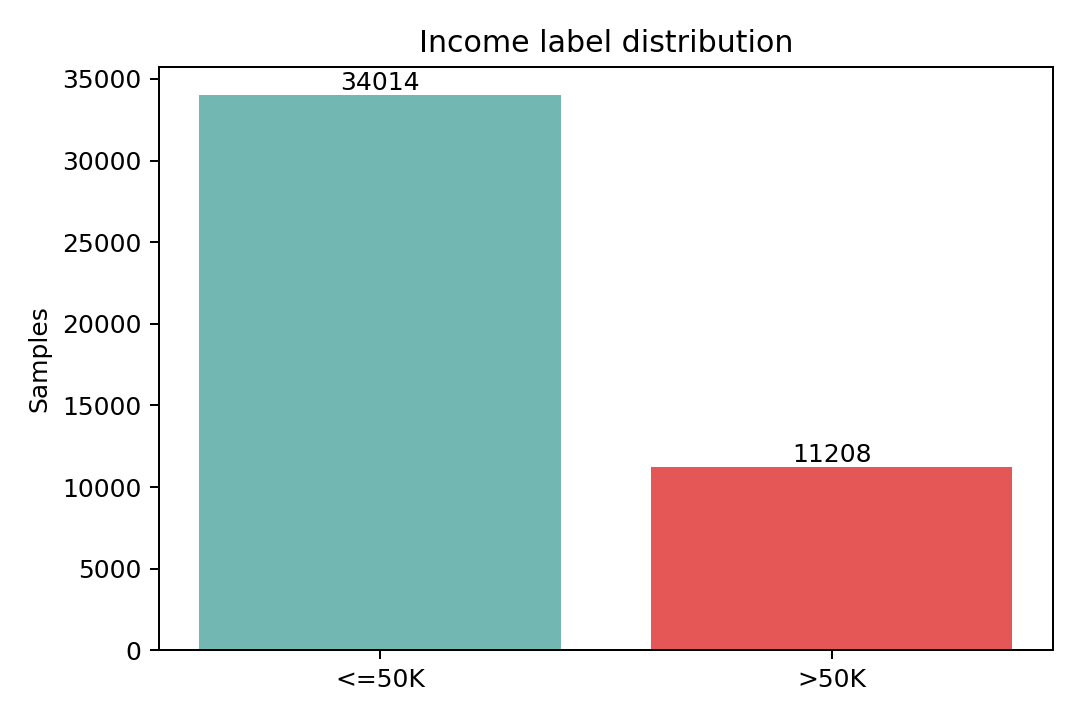
\includegraphics[width=0.6\textwidth]{label_distribution.png}
\caption{收入标签类别分布}
\label{fig:label}
\end{figure}

\begin{figure}[H]
\centering
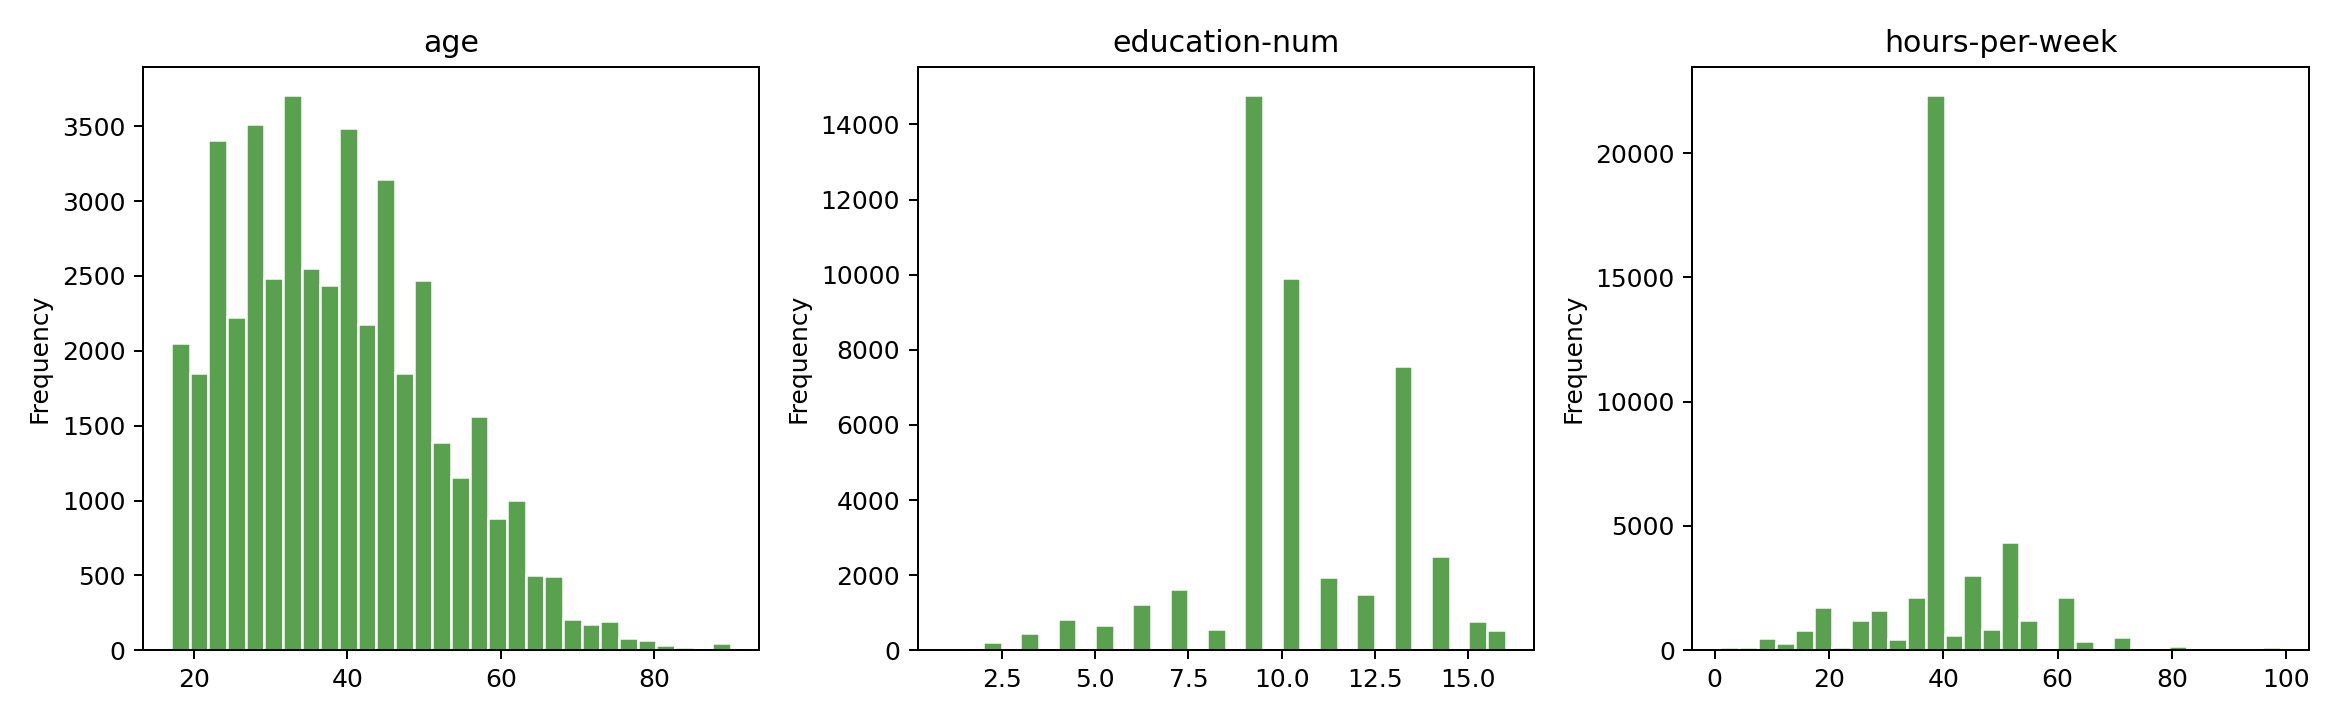
\includegraphics[width=\textwidth]{numeric_feature_histograms.png}
\caption{数值特征分布直方图}
\label{fig:numeric}
\end{figure}

\begin{figure}[H]
\centering
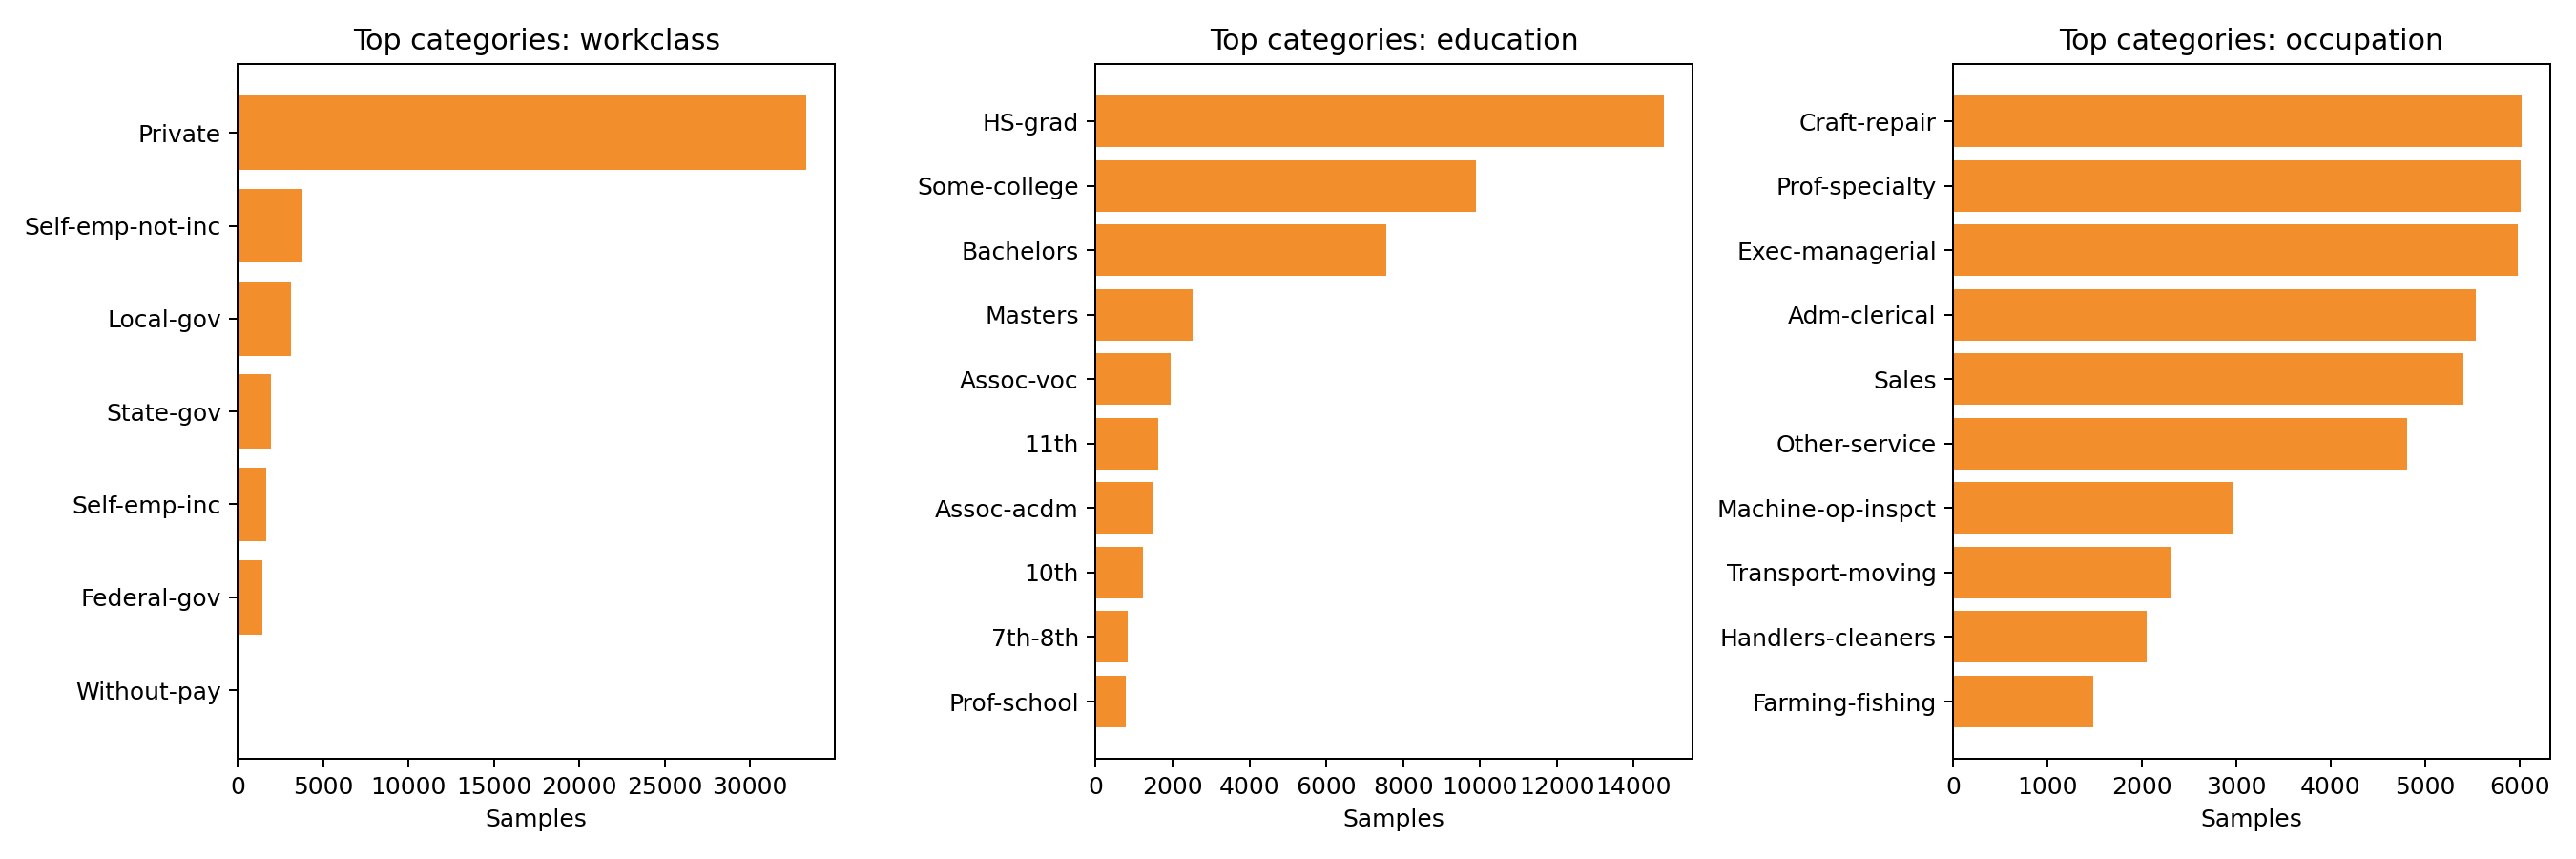
\includegraphics[width=\textwidth]{categorical_feature_distribution.png}
\caption{类别特征 Top-N 分布}
\label{fig:cat}
\end{figure}

\subsection{数据划分与预处理}
我们把清洗后的数据划分为训练集、验证集和测试集，比例为 60\%、20\%、20\%。实际样本数分别为 27,133、9,044 和 9,045。两次划分均使用 \texttt{stratify=y} 和 \texttt{random\_state=42}，保证三个集合中的标签比例接近总体分布。预处理则在划分之后进行：发现 StandardScaler 在训练集数值特征上拟合，OneHotEncoder 在训练集类别特征上拟合，验证集和测试集沿用训练集拟合得到的参数进行 transform。这个顺序能够阻断验证集和测试集统计信息进入训练过程。

\section{实验设计}
实验环境为 Windows，Python 3.11.6，PyTorch 2.11.0+cpu\cite{paszke2019pytorch}，scikit-learn 1.8.0\cite{pedregosa2011scikit}，NumPy 2.4.5，pandas 3.0.0，matplotlib 3.10.8，tqdm 4.67.1。使用 CPU 完成训练。随机种子固定为 42。

baseline 设置为三类。多数类 baseline 将所有测试样本预测为训练集中最多的类别，用来提供类别不均衡情形下的基础参照；随机先验 baseline 按训练集类别比例进行随机预测，用来观察模型相对随机行为的提升幅度；逻辑回归作为线性强基线，用来检验 MLP 引入隐藏层后是否能够获得额外收益。主模型 MLP 使用隐藏层 \texttt{[128,64]}、Dropout 0.3、学习率 0.001、batch size 64、AdamW 优化器和交叉熵损失，训练 50 个 epoch，并保存验证集 Macro-F1 最优的参数。

评价指标包括 Accuracy、Macro Precision、Macro Recall、Macro-F1、Micro-F1 和混淆矩阵。在单标签二分类设置下，Micro-F1 与 Accuracy 数值相同，主要结合 Accuracy 与 Macro-F1 解释整体正确率和少数类识别效果。超参数敏感性分析采用控制变量法：学习率取 0.1、0.01、0.001、0.0001；Dropout 取 0.1、0.3、0.5。每组实验其余参数保持一致，并根据验证集 Macro-F1 判断较优配置。

\section{实验结果与分析}
\subsection{Baseline 与主模型对比}
表\ref{tab:mainresults}给出测试集结果。多数类 baseline 的 Accuracy 为 0.7521，Macro-F1 为 0.4293，该结果对应高收入类别召回率为 0 的预测。随机先验预测 Accuracy 为 0.6312，Macro-F1 约 0.5023，即按照训练集类别比例随机抽样仍会产生大量错误。作为强baseline，逻辑回归取得 0.8456 的 Accuracy 和 0.7777 的 Macro-F1，侧面反映出经过标准化与独热编码处理后，Adult 数据集中的许多特征其实已经具备较好的线性可分性。MLP 在此基础上将 Macro-F1 提升至 0.7947，证实了隐藏层对特征间非线性交互的建模为少数类识别带来了实际增益，例如“学历、工作时长、职业类型”这类联合特征可能比单一特征更具判别价值。

\begin{table}[H]
\centering
\caption{主模型与 baseline 指标对比}
\label{tab:mainresults}
\begin{tabular}{lrrrrr}
\toprule
模型 & Accuracy & Macro Precision & Macro Recall & Macro-F1 & Micro-F1 \\
\midrule
多数类预测 & 0.7521 & 0.3761 & 0.5000 & 0.4293 & 0.7521 \\
随机先验预测 & 0.6312 & 0.5023 & 0.5023 & 0.5023 & 0.6312 \\
逻辑回归 & 0.8456 & 0.8037 & 0.7602 & 0.7777 & 0.8456 \\
MLP & 0.8507 & 0.8030 & 0.7874 & 0.7947 & 0.8507 \\
\bottomrule
\end{tabular}
\end{table}

图\ref{fig:curve}为训练曲线。训练 Loss 与验证 Loss 在前期同步下降，随后进入小幅波动阶段；训练 Accuracy 与验证 Accuracy 的差距较小，模型在训练集和验证集上的拟合状态较为接近。

\begin{figure}[H]
\centering
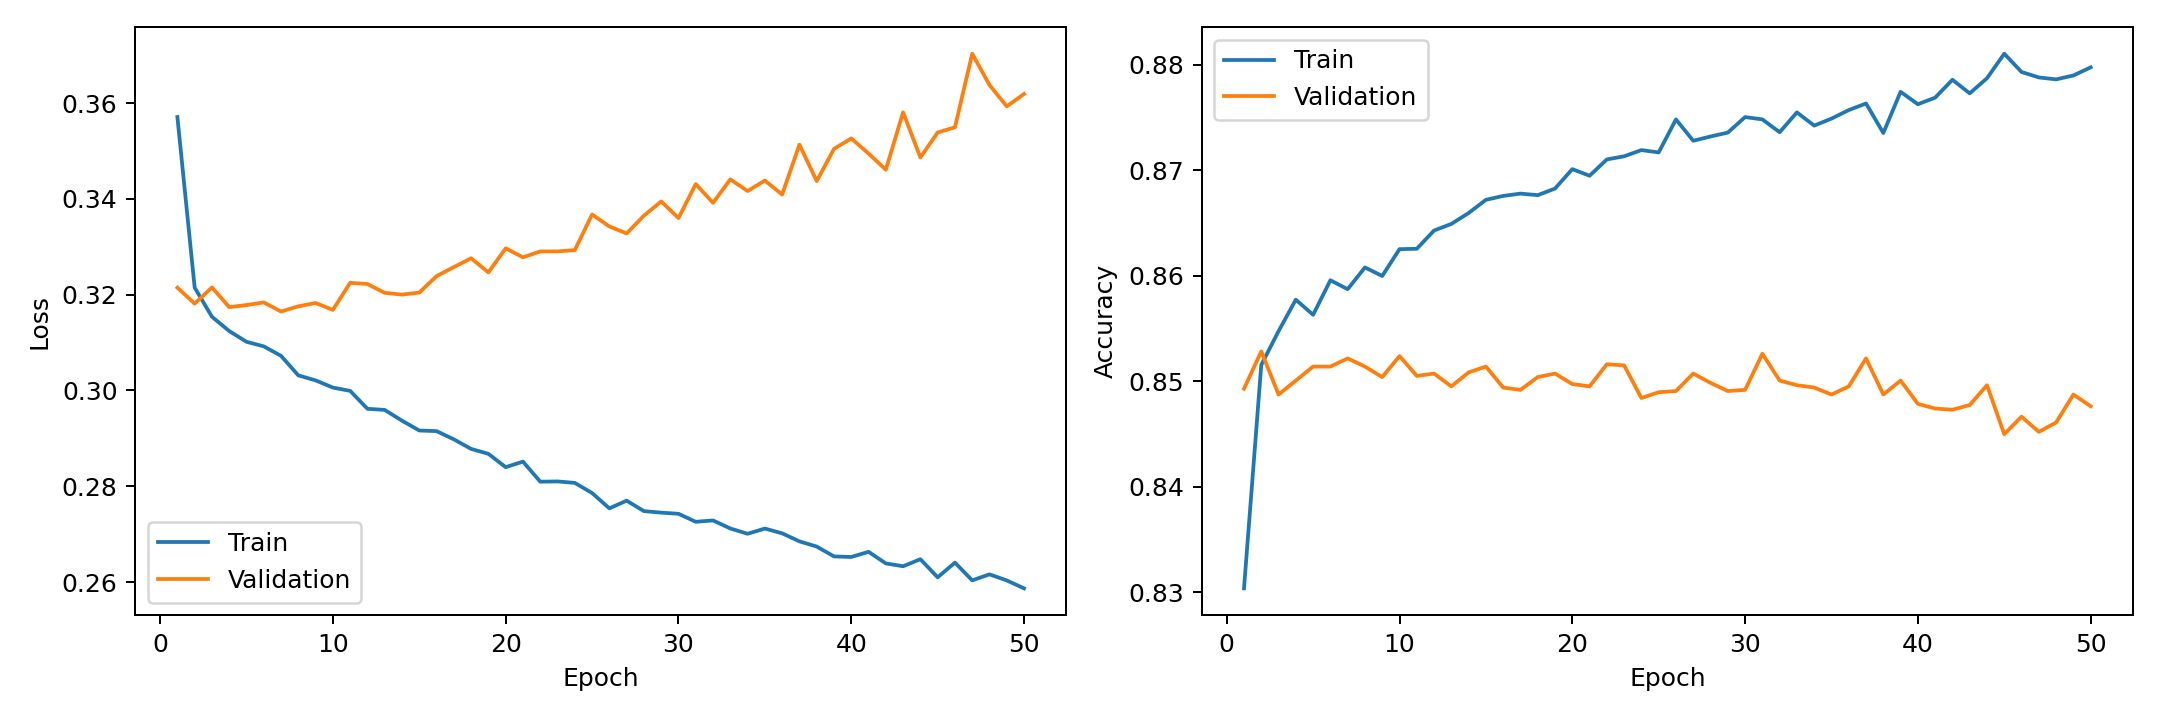
\includegraphics[width=\textwidth]{mlp_training_curves.png}
\caption{MLP 训练与验证 Loss/Accuracy 曲线}
\label{fig:curve}
\end{figure}

\subsection{混淆矩阵与错误分析}
图\ref{fig:cm}显示测试集混淆矩阵。模型对 $\leq 50K$ 类别识别较好，对 $>50K$ 类别仍存在较多漏判，真实高收入样本被预测为低收入。这与类别分布有关：低收入样本约占四分之三，模型在优化整体交叉熵时会更多接触多数类样本，其参数更新也更容易服务于多数类预测。此外，Adult 数据中的特征对收入决定因素的描述存在缺口。地区经济水平、行业细分、职位级别、工作年限、公司规模、资产结构等变量均未进入数据表，因此一些高收入个体可能在现有特征上与低收入个体相似，模型在这类样本上容易产生错误判断。

\begin{figure}[H]
\centering
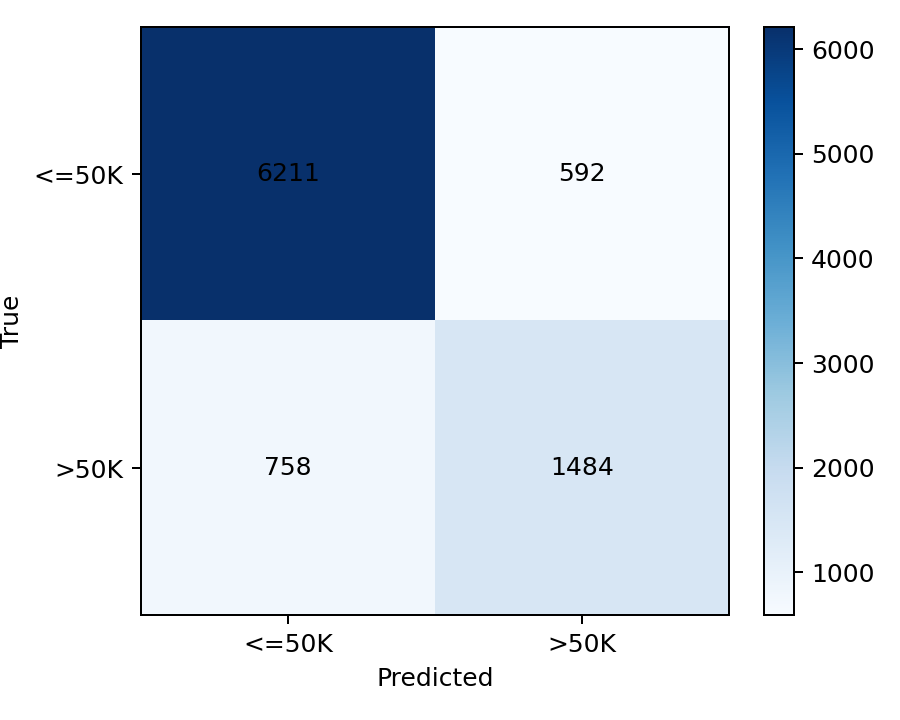
\includegraphics[width=0.55\textwidth]{mlp_confusion_matrix.png}
\caption{MLP 测试集混淆矩阵}
\label{fig:cm}
\end{figure}

\subsection{学习率敏感性分析}
表\ref{tab:lr}和图\ref{fig:lr}展示学习率实验的结果。学习率 0.1 的验证 Macro-F1 为 0.4833，表现明显偏低，反映出参数更新步长过大时优化过程容易产生剧烈波动。学习率 0.01 已经能够得到较好的结果，验证 Macro-F1 为 0.7900。继续将学习率降至 0.001 后，验证 Macro-F1 达到 0.7948，测试 Macro-F1 达到 0.7947。学习率 0.0001 的验证 Accuracy 较高，Macro-F1 和测试 Macro-F1 较低，即在有限 epoch 内，小步长对少数类识别的改善速度不是很明显。

\begin{table}[H]
\centering
\caption{学习率敏感性分析}
\label{tab:lr}
\begin{tabular}{rrrrr}
\toprule
学习率 & 验证 Accuracy & 验证 Macro-F1 & 测试 Accuracy & 测试 Macro-F1 \\
\midrule
0.1 & 0.7653 & 0.4833 & 0.7663 & 0.4882 \\
0.01 & 0.8513 & 0.7900 & 0.8515 & 0.7906 \\
0.001 & 0.8505 & 0.7948 & 0.8507 & 0.7947 \\
0.0001 & 0.8525 & 0.7941 & 0.8500 & 0.7901 \\
\bottomrule
\end{tabular}
\end{table}

\begin{figure}[H]
\centering
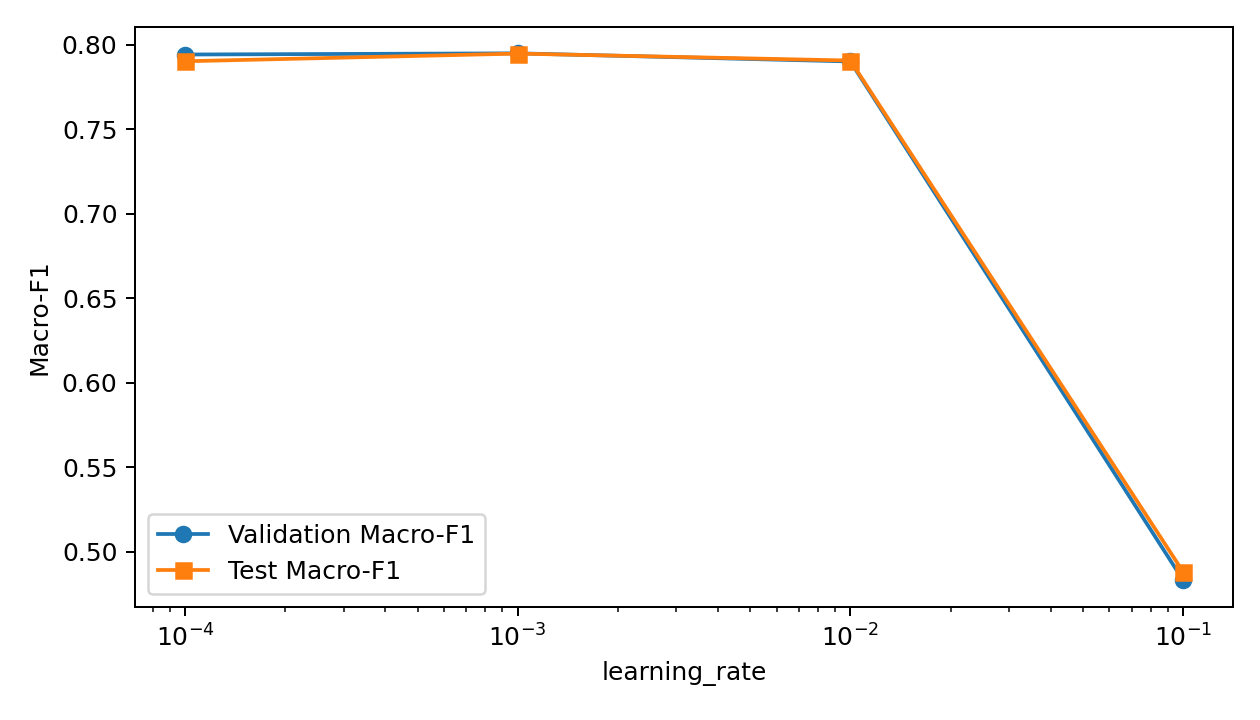
\includegraphics[width=0.75\textwidth]{hparam_lr.png}
\caption{学习率敏感性折线图}
\label{fig:lr}
\end{figure}

\subsection{Dropout 敏感性分析}
表\ref{tab:dropout}和图\ref{fig:dropout}展示 Dropout 实验。Dropout 0.1 的验证 Macro-F1 最高，为 0.7962，测试 Macro-F1 为 0.7861；Dropout 0.3 的测试 Macro-F1 最高，为 0.7947；Dropout 0.5 的验证 Macro-F1 为 0.7950，测试 Macro-F1 为 0.7912。三组结果差距较小，反映 Adult 数据上 MLP 对 Dropout 的响应存在一定波动，随机初始化和训练轮数也会影响单次实验结果。

\begin{table}[H]
\centering
\caption{Dropout 敏感性分析}
\label{tab:dropout}
\begin{tabular}{rrrrr}
\toprule
Dropout & 验证 Accuracy & 验证 Macro-F1 & 测试 Accuracy & 测试 Macro-F1 \\
\midrule
0.1 & 0.8538 & 0.7962 & 0.8475 & 0.7861 \\
0.3 & 0.8505 & 0.7948 & 0.8507 & 0.7947 \\
0.5 & 0.8525 & 0.7950 & 0.8503 & 0.7912 \\
\bottomrule
\end{tabular}
\end{table}

\begin{figure}[H]
\centering
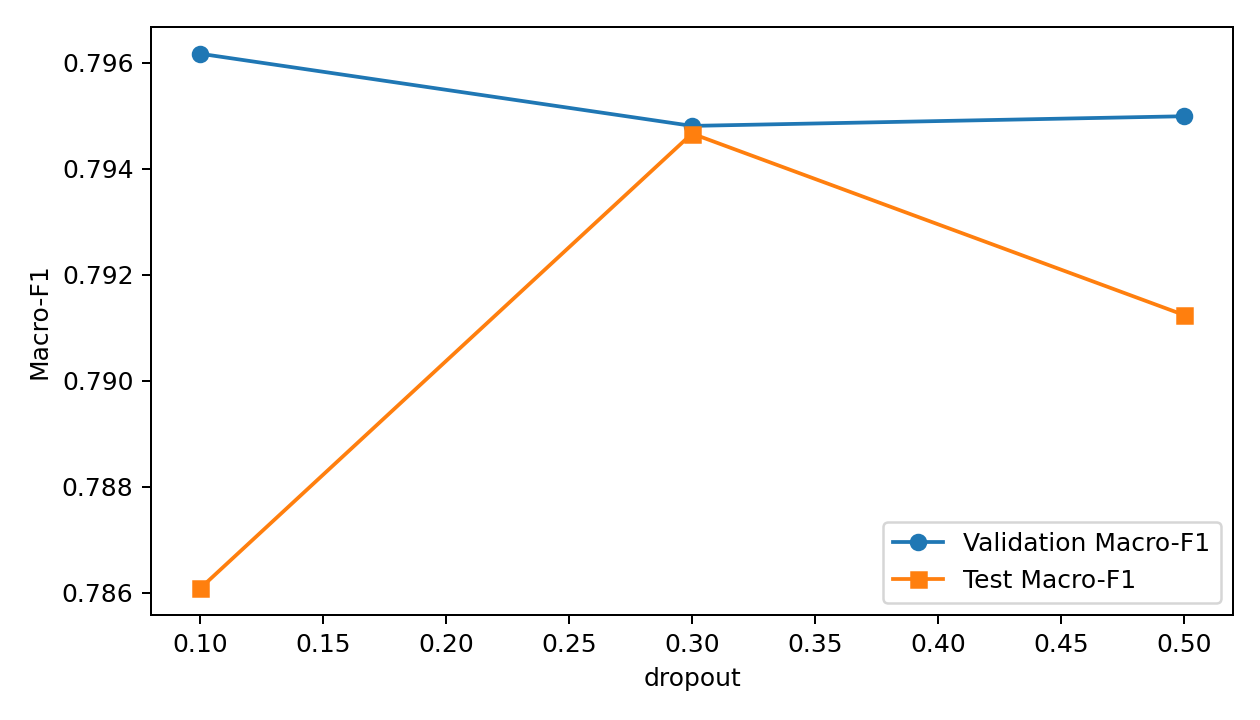
\includegraphics[width=0.75\textwidth]{hparam_dropout.png}
\caption{Dropout 敏感性折线图}
\label{fig:dropout}
\end{figure}

\section{总结与反思}
本次实验围绕 UCI Adult 收入预测任务完成了一个监督学习二分类流程。数据处理阶段从原始文件读取开始，依次完成格式统一、缺失值识别、样本清洗、标签编码和探索性可视化；建模阶段按照 60\%/20\%/20\% 进行分层划分，并将预处理器的拟合过程限定在训练集内；评估阶段则通过多数类预测、随机先验预测和逻辑回归建立参照，再使用 MLP 作为主模型观察非线性建模带来的增益。

实验结果显示，MLP 的 Accuracy 和 Macro-F1 均高于三个参考模型，这表明隐藏层确实学习到了一部分特征组合信息。与此同时，提升幅度保持在较小范围内，这也符合 Adult 数据集的特征特点。该数据集属于结构化表格数据，许多强信号特征经过独热编码后已经可以被线性模型利用；收入本身又受到职位层级、行业细分、地区经济水平等变量影响，而这些高价值信号未能体现在原始字段中。因此，模型性能最终受到特征表达上限、类别不均衡和少数类样本规模的共同约束。

在数据层面，直接删除缺失样本是一种稳妥选择，信息利用率仍有继续提升的空间。后续可以尝试众数插补、缺失类别编码或 KNN 插补等策略，再比较不同清洗方式对 Macro-F1 和少数类召回率的影响。在模型层面，本次对比范围主要集中于逻辑回归和 MLP，随机森林、梯度提升树等模型通常更适合结构化表格数据，将这些方法纳入横向比较，有助于更准确地判断 MLP 在该任务中的实际价值。

此外，本次超参数敏感性分析主要依赖单次运行结果，后续可以引入多组随机种子并报告均值与方差，以减少偶然初始化对结论的影响。收入预测还涉及性别、种族等敏感属性，模型若进入真实决策场景，除了关注 Accuracy 和 Macro-F1，还应继续考察不同群体上的误差差异。围绕这些方向继续扩展，我们能够从单纯记录分数进一步推进到解释模型行为和评估应用边界。

\appendix
\section{项目代码与实验材料}
本报告配套的关键源码、实验结果、图表文件、论文 LaTeX 源码和数据处理产物已整理至 GitHub 仓库：
\[
\url{https://github.com/zt2misay2/AI-Final-Project}
\]
仓库中的 \texttt{src/} 目录保存数据准备、baseline 训练、MLP 训练和超参数分析脚本；\texttt{results/} 目录保存清洗统计、模型指标、训练日志和超参数实验结果；\texttt{figures/} 目录保存论文引用的可视化图表；\texttt{paper/} 目录保存 \LaTeX{} 论文源码与参考文献文件。按照仓库 README 中的运行顺序执行脚本，可以复现实验数据处理、模型训练和图表生成过程。

\bibliographystyle{plain}
\bibliography{references}

\end{document}
